\documentclass[11pt, addpoints]{exam}

\bibliographystyle{abbrv}

\usepackage{amsfonts}

\usepackage{amsthm}

\usepackage{amssymb}

\usepackage{amsmath}

\usepackage{multicol}

\usepackage{enumerate}

\usepackage[all]{xy}

\usepackage{graphicx}

\usepackage{comment}

\RequirePackage{pinlabel}

\usepackage{xcolor}
\usepackage{soul}

\newcommand{\N}{\mathbb{N}}

\newcommand{\Z}{\mathbb{Z}}

\newcommand{\R}{\mathbb{R}}

\newcommand{\Q}{\mathbb{Q}}

\newcommand{\C}{\mathbb{C}}

\newcommand{\T}{\mathbb{T}}

\newcommand{\ra}{~~\Rightarrow~~}

\newcommand{\lra}{~~\Leftrightarrow~~}

\setlength{\unitlength}{1.5cm}

\addpoints

\usepackage{array}
\usepackage{tikz}
\usepackage{pgfplots}
\usepgfplotslibrary{fillbetween}
\usetikzlibrary{patterns}

\tikzset{
  jumpdot/.style={mark=*,solid},
  excl/.append style={jumpdot,fill=white},
  incl/.append style={jumpdot,fill=black},
}

\begin{document}




\section*{Math 241\\
Midterm 1 (make up)\\ 
Fall 2024}

\vspace{0.5in}
\noindent\textbf{Name:} \underline{\hspace{3in}} \\ \\
%\textbf{Section number:} \underline{\hspace{0.3in}} \\ \\

%\noindent If you do not know your section, fill out the following: \\ \\
%\textbf{Instructor:} \underline{\hspace{2in}} \\ \\
%\textbf{TA:} \underline{\hspace{2.55in}} 

\begin{comment}
\hspace{-0.23in}\begin{minipage}{0.75\linewidth}
\noindent\textbf{Draw a circle} around your section number below.\\

\noindent\begin{tabular}{lll}
%\setlength{\extrarowheight}{1in}
%\renewcommand{\arraystretch}{2}
%\rule{0pt}{24pt}
 & TA & Recitation \\
\hline \\[-4pt]
1 & Mona Aschenbrenner & TR	1:30-2:20 \\[8pt]
2 & Janani Lakshmanan & WF 9:30-10:20 \\[8pt]
3 & Mona Aschenbrenner & WF	10:30-11:20 \\[8pt]

\end{tabular}
\end{minipage}
\end{comment}


\begin{center}
\begin{minipage}{0.3\linewidth}
\gradetable[v][questions]  
\end{minipage}   
\end{center}


\vspace{2in}
\begin{itemize}
\item Show all your work neatly.
\item Indicate your final answer by either circling, underlining twice, or boxing your answer.
\item \textbf{This exam is closed book, closed notes.}
\item \textbf{No electronic devices or internet access is allowed.}
\item You have 80 minutes to complete this exam.
\item Good luck!
\end{itemize}

           

\clearpage

\begin{questions}

\question The domain of the functions $f$ and $g$ is the closed interval $[0,4]$ and their graphs are represented below.
\begin{figure}[h!]
	\labellist
	\small
	\pinlabel $f(x)$ at 108 140
	\pinlabel $g(x)$ at 123 115
	\endlabellist
	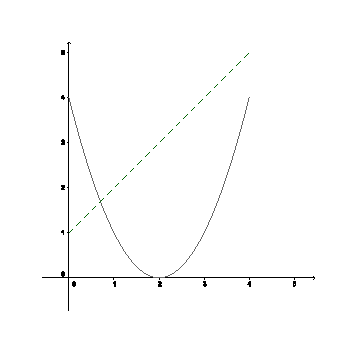
\includegraphics[width=0.6
\textwidth]{1-3-01}
\end{figure}

Determine whether the following compositions are defined. When they are defined, determine their value.
\addpoints
 \begin{parts}
    \part[2] $(g\circ f)(2)$
    \vspace{1in}
    \part[2] $(f\circ f)(2)$
    \vspace{1in}
    \part[2] $(g\circ g)(4)$
    \end{parts}


\pagebreak
         
\question Below is the graph of the function $f(x)$. Find the following.
\vspace{0.25in}
\begin{center}
\includegraphics[scale=0.3]{Images/Sum23M241_MT1_pic1.jpeg}
\end{center}
\addpoints
\begin{parts}
    \part[2] Domain
    \vfill
    \part[2] Interval(s) of increase.
    \vfill
    \part[2] Interval(s) of decrease.
    \vfill
\end{parts}

\clearpage

\question Find the indicated values for the graph of $f(x)$ below. Note that there is a vertical asymptote $x=-1$. If the limit is $-\infty$ or $\infty$, state which. Otherwise, if the limit doesn't exist, write DNE.
\vspace{0.25in}
\begin{center}
\includegraphics[scale=0.35]{Images/Sum23M241_MT1_pic2.jpeg}
\end{center}
\vspace{0.25in}
\begin{parts}
\begin{multicols}{2}
\vspace{0.1in}
\part[1] $\displaystyle\lim_{x\to -1^{-}} f(x)$
\vspace{0.35in}
\part[1] $\displaystyle\lim_{x\to -1^{+}} f(x)$
\vspace{0.35in}
\part[1] $\displaystyle\lim_{x\to -1} f(x)$
\vspace{0.35in}
\part[1] $f(0)$
\vspace{0.35in}

\part[1] $\displaystyle\lim_{x\to 0} f(x)$
\vspace{0.35in}
\part[1] $\displaystyle\lim_{x\to 1^-} f(x)$
\vspace{0.35in}
\part[1] $\displaystyle\lim_{x\to 1^+} f(x)$
\vspace{0.35in}
\part[1] $\displaystyle\lim_{x\to 2} f(x)$
\vspace{0.35in}

\end{multicols}

\part[4] Give the $x$-values where the function $f(x)$ is discontinuous.
\vfill
\part[2] For the removable discontinuity/discontinuities, how can you redefine $f(x)$ to make it continuous there?
\vfill
\end{parts}

\clearpage

\question Compute the following limits. L'Hopital's rule is not allowed.
\addpoints
\begin{parts}
\part[5] $\displaystyle\lim_{x\to 2} \dfrac{x^2+x-6}{x^2-4}$
\vfill


\part[5] $\displaystyle\lim_{x\to 0} \dfrac{\tan(x)}{2x}.$
\vfill
\pagebreak


\part[5] $\displaystyle\lim_{x\to 9} \dfrac{\sqrt{x}-3}{x-9}$
\vfill


\part[5] $\displaystyle\lim_{x\to 3^+} \dfrac{3-x}{|x-3|}$
\vfill

\end{parts}

\pagebreak

\question Use the differentiation rules to compute the derivative of the following. \textbf{Just apply the rules, no need to simplify.}

\addpoints
\begin{parts}
\part[8] $w = (3x^2 - 4x)(x^{1/5} + \sqrt{x})$
\vfill
\part[8] $z = \dfrac{2x^4 - 3x^2 - 7}{x^2-4}$
\vfill
\part[8] $y = (2x+1)^{4}\cos(3x)$
\vfill
\end{parts}

\clearpage

\question We are going to use  the \textbf{definition} of the derivative to compute $f'(t)$ for $$f(t) = \dfrac{1}{3t+1}.$$
\addpoints
\begin{parts}
\part[2] Using the definition of the derivative, write what $f'(t)$ is explicitly as a limit, but \textbf{do not simplify.}
\vspace{0.75in}
\part[8] Find $f'(t)$ by evaluating the limit in your answer from part (b) above. Show that it is equal to $f'(t) = -\dfrac{3}{(3t+1)^2}.$
\vfill
\end{parts}
\clearpage

\question[12] A ladder 10 ft long rests against a vertical wall. If the bottom of the ladder slides away from the wall at a rate of 1 ft/s, how fast is the top of the ladder sliding down the wall when the bottom of the ladder is 6 ft from the wall? 

\pagebreak

\question[8] Use implicit differentiation to find $\frac{dy}{dx}$ for $$x^4-xy+y^5=15$$ at the point $(2,1).$
\end{questions}
    
\end{document}